
\newpage
\section{Casos de uso}
El la siguiente sección se definen y describen los actores, funciones y escenarios, explicando su funcionalidad e interacción con la aplicación.\par
\vspace{5mm}
\begin{figure}[h!]
	\centering
	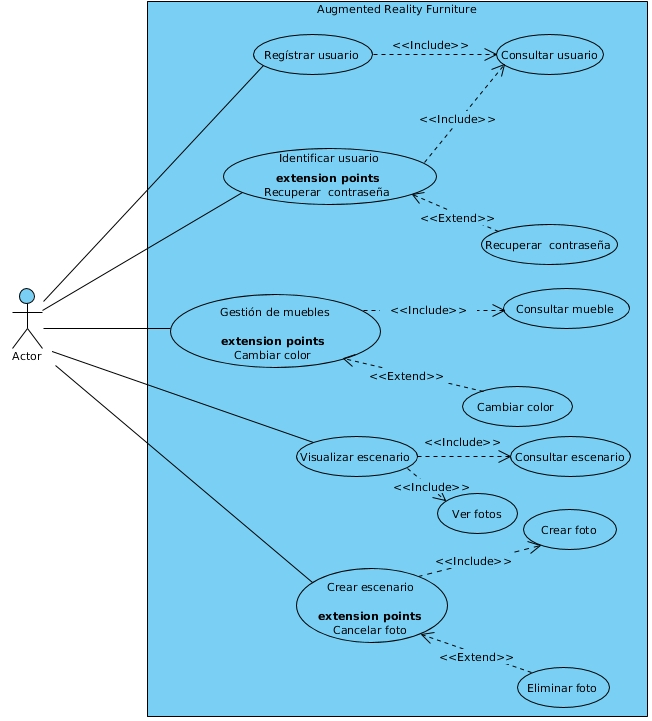
\includegraphics[width=15cm,height=17cm]{imagenes/analisis/casosDeUso.jpg}
	\caption{Casos de uso.}
	\label{fig:analogo}
\end{figure}  
\newpage

\subsection{CU1. Iniciar sesión}\par
Es el escenario de autenticación y acceso de usuario a la aplicación. 
\begin{itemize}
	\item El usuario introduce su usuario y contraseña en los campos de textos mostrados.
	\item El usuario da click en el botón "Iniciar sesión".
	\item Si algún dato es omitido o está mal escrito (por ejemplo, si el campo "usuario" no tiene la estructura de un email) se mostrará un mensaje en pantalla notificando el error.
	\item De no haber errores, el sistema consulta en la base de datos si se encuentra un registro con los datos ingresados por el usuario.
	\item Si encuentra una coincidencia, se muestra el menú principal donde el usuario puede visualizar sus escenarios y proyectos. Si no se encuentra una coincidencia, se muestra un mensaje en pantalla diciendo que los datos ingresados son incorrectos, y la pantalla mostrada seguirá siendo el Login mientras la autenticación no sea exitosa.
\end{itemize}
\begin{figure}[h!]
	\centering
	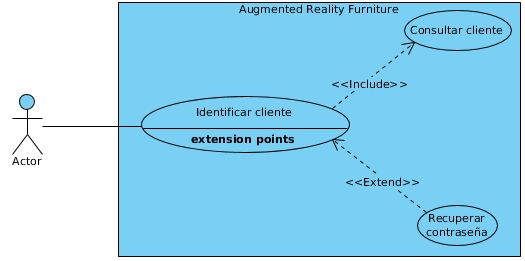
\includegraphics[width=12cm,height=6cm]{imagenes/analisis/login.jpg}
	\caption{CU1 - Login.}
	
	\label{fig:analogo}
\end{figure}  

\subsection{CU2. Registrar cuenta} \par
Es el escenario donde un usuario registra una nueva cuenta para poder tener acceso al sistema.
	\begin{itemize}
		\item En la pantalla inicial, el usuario da click en el botón "Registrar".
		\item Se mostrará una pantalla con un pequeño formulario donde el usuario ingresará sus datos como son: nombre, email y contraseña. La contraseña debe cumplir con la BRX. También habrá un campo adicional donde deberá introducir de nuevo la contraseña para verificar que el usuario la escribió como la pensó inicialmente.
		\item Tras haber llenado esos campos el usuario da click en el botón "Registrar cuenta".
		\item Si hay algún error en el formulario (por ejemplo, el email no tiene la sintaxis que debe tener un email o la contraseña no cumple con la regla de negocio BRX) se mostrará en pantalla a través de un mensaje.
		\item De ser exitoso el proceso anterior, el sistema consulta la base de datos para verificar que se cumpla la regla de negocio BRX. Si no se cumple, un mensaje en pantalla es msotrado diciendo que el correo ya ha sido registrado en otra cuenta. Si es cumplida, el sistema genera un registro de usuario con los datos ingresados.
		\item El sistema muestra en pantalla un mensaje diciendo que el usuario fue creado con éxito y la pantalla mostrada cambia a la inicial donde el usuario puede iniciar sesión con los datos de la cuenta que acaba de crear.
	\end{itemize}
\begin{figure}[h!]
	\centering
	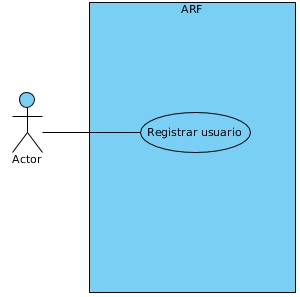
\includegraphics[width=12cm,height=6cm]{imagenes/analisis/registrarUsuario.jpg}
	\caption{CU2 - Registrar usuario.}
	\label{fig:analogo}
\end{figure} 
\newpage
\subsection{CU3. Recuperar cuenta}  \par
Escenario donde un usuario recupera el acceso a una cuenta de la cual olvidó su contraseña
\begin{itemize}
	\item En la pantalla inicial el usuario da click en el botón "Olvidé mi contraseña".
	\item El sistema muestra la pantalla de recuperación de cuenta donde hay un campo donde el usuario debe ingresar el correo con el que registró la cuenta.
	\item El usuario da click en el botón "Enviar código de recuperación".
	\item El sistema verifica que el correo ingresado tenga una estructura correcta. De haber un error en la entrada el sistema lo muestra en un mensaje.
	\item Si la validación es correcta el sistema envía un correo al email ingresado el cual contiene un código de recuperación.
	\item El sistema muestra una pantalla que contiene otro campo donde el usuario debe introducir el código de verificación enviado al correo.
	\item El usuario da click en el botón "Verificar código".
	\item El sistema verifica que el valor ingresado contenga sólo números. De haber un error en la entrada el sistema lo muestra en un mensaje.
	\item Tras la verificación anterior exitosa, el sistema verifica que el código ingresado sea el mismo que se generó y envío al correo. De ser incorrecto el sistema lo notifica en pantalla a través de un correo.
	\item Si el código ingresado coincide, entonces el sistema muestra una pantalla que tiene dos campos para contraseña. En el primer campo el usuario debe introducir una nueva contraseña, la cual debe cumplir con la regla de negocio BRX. En el segundo campo debe volver a escribir la misma contraseña.
	\item El usuario da click en el botón "Actualizar contraseña"
	\item El sistema valida que la contraseña cumpla con la regla de negocio BRX, de no ser así, lo notifica en pantalla a través de un mensaje.
	\item El sistema cambia la contraseña del usuario por la que acaba de ingresar. Tras esto la pantalla muestra un mensaje diciendo si la actualización fue exitosa o no.
	\item De ser exitosa, la pantalla mostrada vuelve a ser la del Login inicial donde el usuario podrá iniciar sesión con su correo y la nueva contraseña.
\end{itemize}
\begin{figure}[h!]
	\centering
	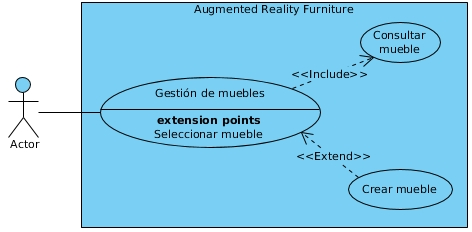
\includegraphics[width=12cm,height=6cm]{imagenes/analisis/seleccionarMueble.jpg}
	\caption{CU3 - Gestión de muebles.}
	\label{fig:analogo}
\end{figure}

\subsection{CU4. Crear proyecto}\par
Escenario donde un usuario crea un proyecto para poder guardar escenarios dentro de él.\par
\textbf{Precondición:} Haber iniciado sesión correctamente.\par
\begin{itemize}
	\item Dentro del menú principal, el usuario da click en la opción "Crear proyecto".
	\item El sistema muestra un formulario donde muestra campos para introducir los siguientes datos: nombre de cliente y observaciones generales del mismo.
	\item El usuario da click en el botón "Crear proyecto".
	\item El sistema verifica que los campos introducidos contengan solamente números, letras y caracteres especiales. De no ser así, el sistema lo notifica en pantalla a través de un mensaje.
	\item El sistema registra en la base de datos un proyecto y lo asocia al usuario que solicita su creación.
	\item El sistema muestra en pantalla un mensaje diciendo si la creación del proyecto fue exitosa o no.
	\item De ser correcta la creación del proyecto, la pantalla mostrada vuelve a ser el menú principal, donde el usuario podrá ver el proyecto creado dando click en el botón "Ver proyectos"
\end{itemize}
\begin{figure}[h!]
	\centering
	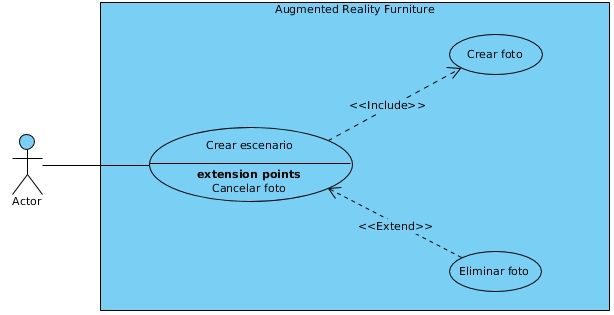
\includegraphics[width=12cm,height=6cm]{imagenes/analisis/crearEscenario.jpg}
	\caption{CU4 - Crear escenario.}
	\label{fig:analogo}
\end{figure}

\newpage
\subsection{CU5 Visualizar escenario}\par
En esta parte el usuario podrá ver las imágenes de un escenario generado con anterioridad, podrá seleccionarlo desde una lista con sus escenarios disponibles
\begin{figure}[h!]
	\centering
	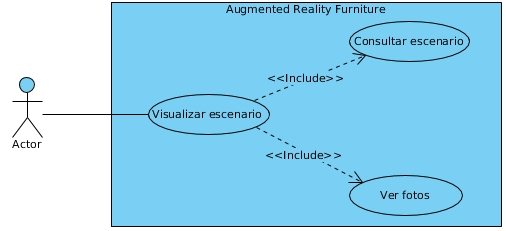
\includegraphics[width=12cm,height=6cm]{imagenes/analisis/visualizarEscenario.jpg}
	\caption{CU5 - Visualizar escenario.}
	\label{fig:analogo}
\end{figure}